%==============================================================================
\chapter{Methodology}
\label{chap:methodology}
%==============================================================================

This chapter describes the implementation used to study automated algorithm
design under stochastic fitness evaluation. The method builds on the Large
Language Model Evolutionary Algorithm (LLaMEA), in which a language model
generates executable optimization algorithms and iteratively modifies them
using information obtained from their evaluation \cite{LLaMEA2024}. In this
thesis, the LLaMEA process is combined with a controlled stochastic
evaluation environment and locally executed large language models (LLMs).

A central methodological distinction is made between the optimization
environment experienced by a generated algorithm and the information used by
the outer synthesis framework to assess that algorithm. During execution, a
generated optimizer interacts with the optimization problem only through the
provided objective interface. Under stochastic conditions, this interface
returns noisy objective values. The optimizer does not receive access to the
analytical benchmark function, the clean objective, or the known optimum.

After the optimizer terminates, the surrounding synthesis framework evaluates
the returned solution using the clean objective. This separation is deliberate.
The stochastic objective defines the information available to the inner
optimization procedure, whereas the clean objective provides a stable
algorithm-level criterion for the outer LLaMEA process. The clean objective is
therefore available to the synthesis framework but not to the generated
optimizer while it performs its search.

The complete methodology consists of a sequence of connected stages. A
continuous black-box optimization problem is first defined together with its
fitness evaluation setup and selected prompt configuration. The resulting
optimization environment is supplied to the LLaMEA synthesis process, where
the LLM generates executable optimization heuristics. The candidates are
extracted, validated, executed, and evaluated by the surrounding framework.
The outer synthesis controller compares the generated algorithms using the
clean quality of the solutions they return and incorporates the evaluation
outcome into the context used for subsequent generations.

When a synthesis run terminates, its final incumbent is retained as the
algorithm produced by that run. The retained algorithms are subsequently
evaluated independently under the experimental conditions defined for the
study. The independent evaluation includes both clean and stochastic fitness
conditions so that the behavior of the generated algorithms can be examined
under different evaluation environments. The resulting measurements are then
used for statistical analysis and comparison with established optimization
algorithms.

Figure~\ref{fig:methodology_architecture} summarizes the complete methodology.
It should be read as a high-level system overview rather than as a
representation of the individual operations inside the LLaMEA evolutionary
loop.

\begin{figure}[htbp]
    \centering
    \resizebox{\textwidth}{!}{%
        \begin{tikzpicture}[
    font=\footnotesize,
    >=Stealth,
    % ---------------------------------------------------------------
    % Global Styling & Dimensions
    % ---------------------------------------------------------------
    baseNode/.style={
        rectangle,
        draw=black!80,
        thick,
        rounded corners=4pt,
        align=center,
        inner sep=7pt
    },
    wideNode/.style={
        baseNode,
        text width=12.2cm
    },
    stageNode/.style={
        baseNode,
        fill=blue!5,
        text width=12.2cm,
        minimum height=1.15cm
    },
    evalBranch/.style={
        baseNode,
        fill=blue!10,
        text width=5.6cm,
        minimum height=1.15cm
    },
    arrow/.style={
        ->,
        >=Stealth,
        thick,
        draw=black!75
    },
    branchArrow/.style={
        ->,
        >=Stealth,
        thick,
        draw=black!65
    }
]

    % ==================================================================
    % 1. EXPERIMENTAL INPUT
    % ==================================================================
    \node[wideNode, fill=yellow!15] (problem) {
        \textbf{Optimization Problem and Experimental Setup} \\[2pt]
        \scriptsize
        Continuous black-box optimization \quad $\bullet$ \quad
        BBOB benchmark functions \quad $\bullet$ \quad
        Dimension $D$ \quad $\bullet$ \quad
        Evaluation budget $B$
    };

    % ==================================================================
    % 2. UNIFIED PROMPT SCAFFOLDING BLOCK
    % ==================================================================
    \node[
        wideNode,
        fill=orange!10,
        draw=orange!80!black,
        below=0.9cm of problem
    ] (promptScaffolding) {
        \textbf{Prompt Scaffolding Framework} \\[2pt]
        \scriptsize
        Invariant layout, API templates, and defensive constraints \\
        coupled with $3 \times 4$ factorial synthesis conditions:
        information modes ($\textsc{Clean}, \textsc{Implicit}, \textsc{Noisy}$)
        $\times$ search strategy scaffolds
    };

    % ==================================================================
    % 3. LLAMEA SYNTHESIS
    % ==================================================================
    \node[
        stageNode,
        below=0.9cm of promptScaffolding
    ] (synthesis) {
        \textbf{LLaMEA Algorithm Synthesis} \\[2pt]
        \scriptsize
        Iterative LLM-driven generation, validation, execution, and semantic selection of candidate heuristics
    };

    % ==================================================================
    % 4. SYNTHESIS OUTPUT
    % ==================================================================
    \node[
        stageNode,
        below=0.85cm of synthesis
    ] (champions) {
        \textbf{Synthesized Algorithms} \\[2pt]
        \scriptsize
        Retained candidate optimization algorithms and corresponding generational telemetry
    };

    % ==================================================================
    % 5. INDEPENDENT EVALUATION HARNESS
    % ==================================================================
    \node[
        stageNode,
        below=0.85cm of champions
    ] (evaluation) {
        \textbf{Independent Algorithm Evaluation} \\[2pt]
        \scriptsize
        Systematic validation of synthesized heuristics across target benchmark environments
    };

    % ==================================================================
    % 6. DUAL EVALUATION BRANCHES (CLEAN & NOISY)
    % ==================================================================
    \node[
        evalBranch,
        below left=0.8cm and 0.25cm of evaluation.south,
        anchor=north east
    ] (cleanEvaluation) {
        \textbf{Clean Evaluation} \\[2pt]
        \scriptsize
        Performance on underlying deterministic BBOB objectives
    };

    \node[
        evalBranch,
        below right=0.8cm and 0.25cm of evaluation.south,
        anchor=north west
    ] (noisyEvaluation) {
        \textbf{Noisy Evaluation} \\[2pt]
        \scriptsize
        Performance under heteroscedastic stochastic observations
    };

    % ==================================================================
    % 7. STATISTICAL ANALYSIS
    % ==================================================================
    \coordinate (evalMid) at ($(cleanEvaluation.south)!0.5!(noisyEvaluation.south)$);

    \node[
        wideNode,
        fill=purple!10,
        below=0.85cm of evalMid
    ] (analysis) {
        \textbf{Statistical Analysis and Comparison} \\[2pt]
        \scriptsize
        Target precision trajectories, empirical runtime distributions (ECDF), and reference benchmark comparisons
    };

    % ==================================================================
    % 8. FINAL RESULTS
    % ==================================================================
    \node[
        wideNode,
        fill=green!15,
        below=0.85cm of analysis
    ] (results) {
        \textbf{Experimental Results and Research-Question Analysis} \\[2pt]
        \scriptsize
        Comparative assessment against CMA-ES, DE, and PSO to address core research questions
    };

    % ==================================================================
    % PIPELINE CONNECTORS
    % ==================================================================
    \draw[arrow] (problem) -- (promptScaffolding);
    \draw[arrow] (promptScaffolding) -- (synthesis);
    \draw[arrow] (synthesis) -- node[fill=white, inner sep=2pt, font=\scriptsize\bfseries] {Synthesized Candidates} (champions);
    \draw[arrow] (champions) -- (evaluation);

    % Dual Evaluation Forks
    \draw[branchArrow] (evaluation.south) -- ++(0,-0.3) -| (cleanEvaluation.north);
    \draw[branchArrow] (evaluation.south) -- ++(0,-0.3) -| (noisyEvaluation.north);

    % Dual Evaluation Convergence into Analysis
    \draw[branchArrow] (cleanEvaluation.south) -- ++(0,-0.3) -| ([xshift=-3.0cm]analysis.north);
    \draw[branchArrow] (noisyEvaluation.south) -- ++(0,-0.3) -| ([xshift=3.0cm]analysis.north);

    \draw[arrow] (analysis) -- (results);

    % ==================================================================
    % STAGE GROUPING CONTAINERS (BACKGROUND)
    % ==================================================================
    \begin{scope}[on background layer]
        % Synthesis Stage Container
        \node[
            draw=blue!50!black,
            dashed,
            fill=blue!2,
            rounded corners=6pt,
            inner sep=9pt,
            fit=(synthesis) (champions),
            label={[font=\scriptsize\bfseries, text=blue!60!black]left:Synthesis}
        ] (synthesisGroup) {};

        % Independent Evaluation Container
        \node[
            draw=blue!50!black,
            dashed,
            fill=blue!2,
            rounded corners=6pt,
            inner sep=9pt,
            fit=(evaluation) (cleanEvaluation) (noisyEvaluation),
            label={[font=\scriptsize\bfseries, text=blue!60!black]left:Evaluation}
        ] (evaluationGroup) {};

        % Analysis Stage Container
        \node[
            draw=purple!60!black,
            dashed,
            fill=purple!2,
            rounded corners=6pt,
            inner sep=9pt,
            fit=(analysis) (results),
            label={[font=\scriptsize\bfseries, text=purple!70!black]left:Analysis}
        ] (analysisGroup) {};
    \end{scope}

\end{tikzpicture}
    }
    \caption{High-level architecture of the methodology used in this thesis.
    The Problem and Fitness Setup, together with the selected prompt
    configuration, define the environment supplied to the LLaMEA synthesis
    stage. LLaMEA produces executable optimization algorithms, which are
    subsequently evaluated independently under clean and stochastic fitness
    conditions and compared with established optimization baselines. The
    resulting measurements are used for statistical and research-question
    analysis.}
    \label{fig:methodology_architecture}
\end{figure}

For reproducibility, the methodology distinguishes between the logical
components of the synthesis framework and their experimental configuration.
The logical components define how objective values are exposed to generated
optimizers, how candidates are generated and validated, how programs are
executed, how candidate quality is measured, and how the evolutionary state
is updated. Quantities such as the number of generations, synthesis budget,
model variant, benchmark functions, dimensions, noise levels, execution
limits, and benchmark repetitions are experimental parameters and are
specified in Chapter~\ref{chap:experiments}.


%==============================================================================
\section{Problem and Fitness Setup}
\label{sec:problem_evaluation_setup}
%==============================================================================

The generated optimizer interacts with the optimization problem only through
the objective interface provided by the evaluation framework. This interface
determines the fitness value observed by the optimizer for each queried
solution. In the deterministic setting, this value corresponds to the clean
objective. In the stochastic setting, the returned fitness additionally
contains a random component.

The purpose of this design is to study how generated optimization algorithms
behave when the fitness information available during search is uncertain
without changing the underlying optimization problem itself. Stochasticity is
therefore introduced at the objective interface rather than by modifying the
generated optimization algorithm.

The outer framework deliberately retains access to the clean objective because
the methodology separates two levels of optimization. At the inner level, a
generated algorithm must solve the black-box optimization problem using only
the evaluations returned by its supplied objective interface. At the outer
level, LLaMEA evolves complete optimization algorithms and therefore requires a
common algorithm-level criterion for comparing generated programs. The clean
objective is used for this outer comparison after the inner optimization run
has finished. It is never provided to the generated optimizer as an additional
objective observation.


%------------------------------------------------------------------------------
\subsection{Fitness Models}
\label{subsec:deterministic_stochastic}
%------------------------------------------------------------------------------

Let $f_{\mathrm{clean}}(x)$ denote the underlying benchmark objective function
for a candidate solution $x \in \mathbb{R}^{D}$. Let $x^*$ denote a global
optimum and let

\begin{equation}
f^* = f_{\mathrm{clean}}(x^*)
\label{eq:true_optimum}
\end{equation}

denote the corresponding optimal objective value. The value $f^*$ is used
internally by the evaluation framework when constructing the stochastic
objective. It is not exposed to the generated optimizer.

For deterministic evaluation, the fitness returned to the optimizer is simply

\begin{equation}
f_{\mathrm{obs}}(x) = f_{\mathrm{clean}}(x).
\label{eq:deterministic_objective}
\end{equation}

Under stochastic evaluation, the observed fitness is instead defined as

\begin{equation}
f_{\mathrm{obs}}(x) = f_{\mathrm{clean}}(x) + z,
\label{eq:stochastic_objective}
\end{equation}

where $z$ is a random perturbation.

Two additive Gaussian formulations were considered when designing the
stochastic evaluation environment. The first is a homoscedastic formulation
whose noise scale is calibrated once from the overall scale of the objective.
The second is a heteroscedastic formulation whose noise scale changes
according to the clean optimality gap of the queried point.


%..............................................................................
% Homoscedastic formulation
%..............................................................................

For the homoscedastic formulation, a characteristic problem scale is estimated
before optimization. A set of $N$ points is sampled uniformly from the bounded
search space,

\begin{equation}
x_i \sim \mathcal{U}(\mathrm{lb},\mathrm{ub}),
\qquad i = 1,\ldots,N.
\end{equation}

The mean absolute difference between the sampled clean objective values and
the known optimum is then calculated as

\begin{equation}
s_{\mathrm{landscape}}
=
\frac{1}{N}
\sum_{i=1}^{N}
\left|
f_{\mathrm{clean}}(x_i) - f^*
\right|.
\label{eq:landscape_scale}
\end{equation}

The standard deviation used for the complete optimization problem is

\begin{equation}
\sigma_{\mathrm{hom}}
=
\sigma s_{\mathrm{landscape}},
\label{eq:homoscedastic_std}
\end{equation}

where $\sigma$ controls the requested noise intensity.

The resulting noisy observation follows

\begin{equation}
f_{\mathrm{obs}}(x)
\sim
\mathcal{N}
\left(
f_{\mathrm{clean}}(x),
\sigma_{\mathrm{hom}}^2
\right).
\label{eq:homoscedastic_noise}
\end{equation}

Calibrating the perturbation to the problem scale avoids applying the same
absolute noise magnitude to benchmark functions with substantially different
objective scales. Once the calibration has been performed, however,
$\sigma_{\mathrm{hom}}$ remains constant for every objective query of the same
problem.

A point far from the optimum and a point already close to the optimum
therefore receive perturbations drawn using the same absolute standard
deviation. This behavior represents a valid stochastic assumption, but it is
not the assumption selected for the final stochastic environment in this
thesis.

The intended experimental setting requires the magnitude of the perturbation
to change with the remaining optimization error. Under the homoscedastic
formulation, the absolute noise level remains fixed even when the clean
objective gap changes substantially. A perturbation that is moderate relative
to the objective error in one part of the search can therefore become large
relative to the remaining error closer to the optimum.


%..............................................................................
% Heteroscedastic formulation
%..............................................................................

For the final stochastic evaluation model, the standard deviation is instead
determined separately for each queried point. The dynamic standard deviation
is defined as

\begin{equation}
\sigma_{\mathrm{dynamic}}(x)
=
\sigma
\left|
f_{\mathrm{clean}}(x) - f^*
\right|.
\label{eq:dynamic_noise_std}
\end{equation}

The perturbation is sampled according to

\begin{equation}
z
\sim
\mathcal{N}
\left(
0,
\sigma_{\mathrm{dynamic}}^2(x)
\right).
\label{eq:proportional_gaussian_noise}
\end{equation}

The noisy observation therefore becomes

\begin{equation}
f_{\mathrm{obs}}(x)
=
f_{\mathrm{clean}}(x) + z.
\label{eq:heteroscedastic_objective}
\end{equation}

The resulting objective is heteroscedastic because the variance of the
observed fitness depends on the queried point. Larger clean objective gaps
produce larger perturbation scales, whereas the standard deviation decreases
as the clean objective approaches $f^*$.

For $\sigma = 0$, the perturbation vanishes and the evaluation becomes
deterministic.

Using the optimality gap rather than the raw objective value also avoids
making the stochastic scale dependent on an arbitrary vertical translation of
the objective. Suppose that the objective is shifted by a constant $c$,

\begin{equation}
\tilde{f}(x)
=
f_{\mathrm{clean}}(x) + c,
\end{equation}

and that the corresponding optimum is

\begin{equation}
\tilde{f}^{*}
=
f^* + c.
\end{equation}

The resulting optimality gap remains unchanged:

\begin{equation}
\left|
\tilde{f}(x) - \tilde{f}^{*}
\right|
=
\left|
f_{\mathrm{clean}}(x) - f^*
\right|.
\end{equation}

The stochastic scale is therefore unaffected by a common vertical shift of
the objective.

The behavior of the heteroscedastic formulation can also be illustrated
numerically. For an illustrative value of $\sigma = 0.1$, a point with an
objective gap of approximately $10^3$ produces

\begin{equation}
\sigma_{\mathrm{dynamic}}
=
0.1 \cdot 10^3
=
10^2.
\label{eq:dynamic_std_example_large}
\end{equation}

For a point whose objective gap is approximately $10^1$, the corresponding
standard deviation becomes

\begin{equation}
\sigma_{\mathrm{dynamic}}
=
0.1 \cdot 10^1
=
10^0.
\label{eq:dynamic_std_example_small}
\end{equation}

These values are used only to illustrate the scaling rule. The actual noise
parameters used in the experiments are reported in
Chapter~\ref{chap:experiments}.


%..............................................................................
% Repeated stochastic observations
%..............................................................................

The stochastic realization is associated with the objective query rather than
being permanently attached to a coordinate. Each query obtains a new sample
from the corresponding noise distribution.

For repeated evaluations of the same coordinate $x$, the clean objective and
conditional noise distribution remain unchanged, but the realized
perturbations can differ:

\begin{equation}
f_{\mathrm{obs}}^{(i)}(x)
=
f_{\mathrm{clean}}(x) + z_i,
\label{eq:independent_noise_realizations}
\end{equation}

with

\begin{equation}
z_i
\sim
\mathcal{N}
\left(
0,
\sigma_{\mathrm{dynamic}}^2(x)
\right).
\end{equation}

Thus, repeated evaluations of the same coordinate can produce different
observed fitness values.

This property matters because generated optimizers can rely on rankings,
direct fitness comparisons, progress estimates, or stored objective values
when making search decisions. If two candidate points have similar clean
objective values, a particular stochastic realization can temporarily reverse
their observed ranking and thereby change the subsequent search trajectory.

The random-number generation used by the objective wrapper is kept separate
from the clean objective calculation. Reproducibility of stochastic
experiments is obtained through the configured random-seed policy. The exact
seed values and run-level seed configuration are reported in
Chapter~\ref{chap:experiments}.


%..............................................................................
% Clean post-execution assessment
%..............................................................................

After a generated optimizer has exhausted its evaluation budget or otherwise
completed its search, the evaluation framework uses the returned
$x_{\mathrm{best}}$ to calculate the clean optimality gap

\begin{equation}
\Delta f(x_{\mathrm{best}})
=
\left|
f_{\mathrm{clean}}(x_{\mathrm{best}}) - f^*
\right|.
\label{eq:clean_optimality_gap}
\end{equation}

This calculation is performed outside the evaluation budget provided to the
generated optimizer. It does not create an additional objective observation
that can influence the optimizer's search.

The stochastic observations and the clean diagnostic value therefore have
different roles. The stochastic objective determines the search trajectory of
the generated optimizer and consequently affects which solution it returns.
The clean diagnostic value is calculated only after execution and is used by
the outer LLaMEA process to assess the quality of the returned solution.

This deliberate separation prevents a favorable individual noise realization
from being used directly as the algorithm-level selection criterion while
preserving a stochastic search environment for the generated optimizer.


%------------------------------------------------------------------------------
\subsection{Noise Model Examples}
\label{subsec:noise_model_illustration}
%------------------------------------------------------------------------------

The behavior of the stochastic formulations is illustrated together with the
underlying clean objective on two BBOB benchmark functions. Each visualization
contains three representations of the same problem: the clean objective, the
homoscedastic additive model, and the heteroscedastic optimality-gap model.

Showing all three representations makes the difference between a fixed
stochastic scale and a query-dependent stochastic scale visible while keeping
the underlying benchmark function unchanged.

The first example is the Rosenbrock function $f_8$, which contains a narrow
curved valley \cite{Hansen2010}. Its structure makes it useful for examining
how the two noise models behave when objective values differ substantially
between poor regions of the search space and points closer to the optimum.

Under the homoscedastic formulation, the scale estimated before optimization
determines one fixed noise standard deviation for the complete problem. The
absolute perturbation scale therefore remains the same when a queried point
moves from a region with a large objective error toward a region with a much
smaller error.

The heteroscedastic formulation behaves differently. Its standard deviation
is recomputed from the clean optimality gap for each query. Regions with large
objective gaps therefore exhibit larger stochastic variation, whereas the
perturbation magnitude decreases as the clean objective approaches the
optimum.

The clean representation serves as the reference against which both stochastic
formulations can be compared.

\begin{figure}[htbp]
    \centering

    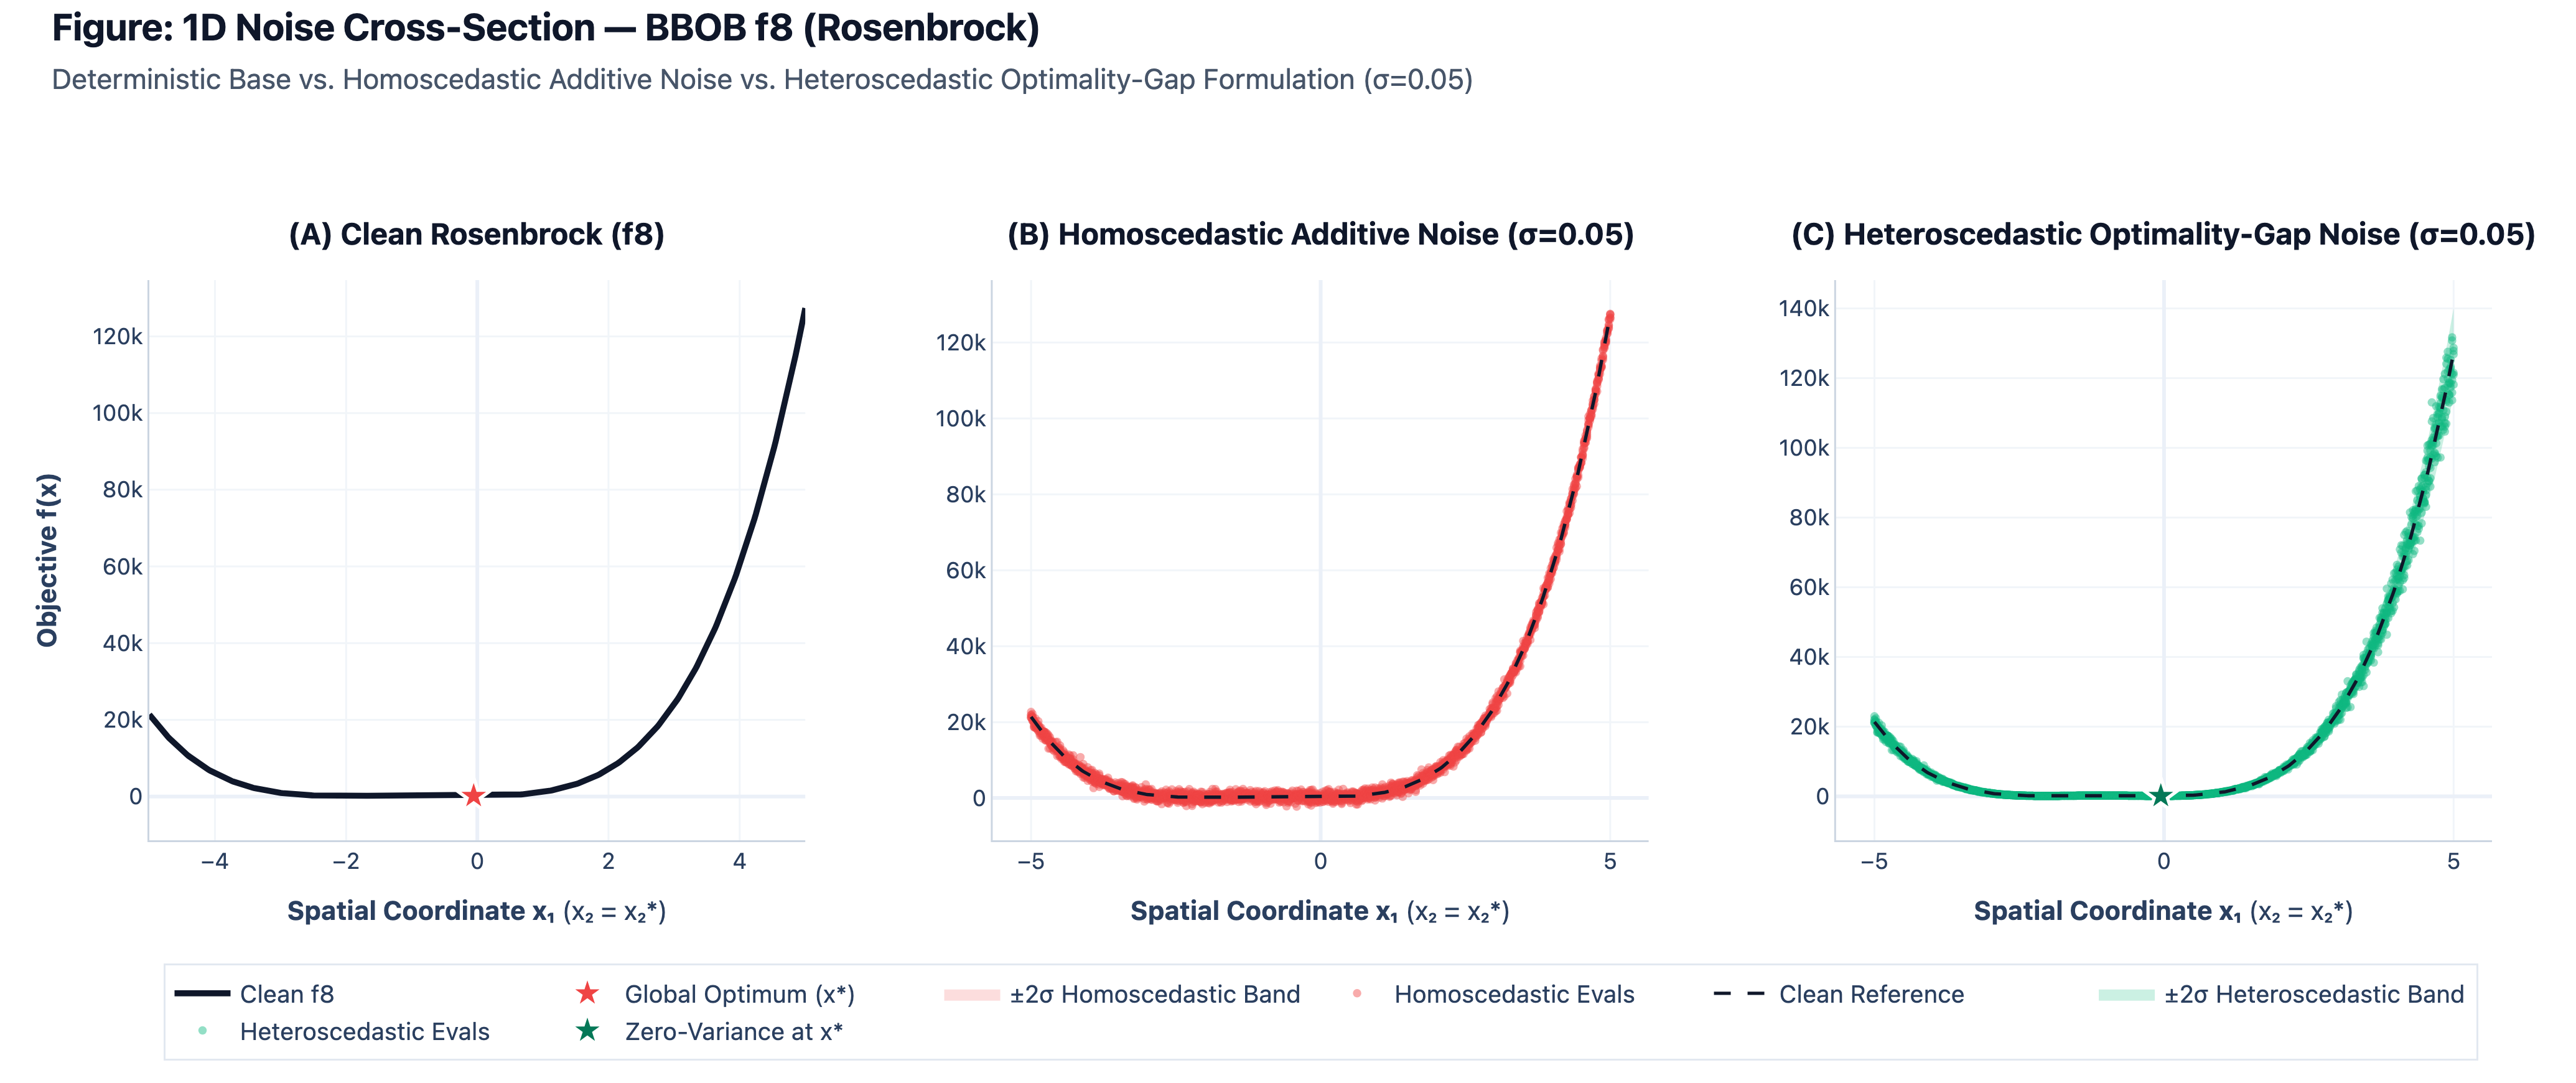
\includegraphics[width=\textwidth]
    {images/f8/figure_1d_noise_cross_section.png}

    \vspace{0.4cm}

    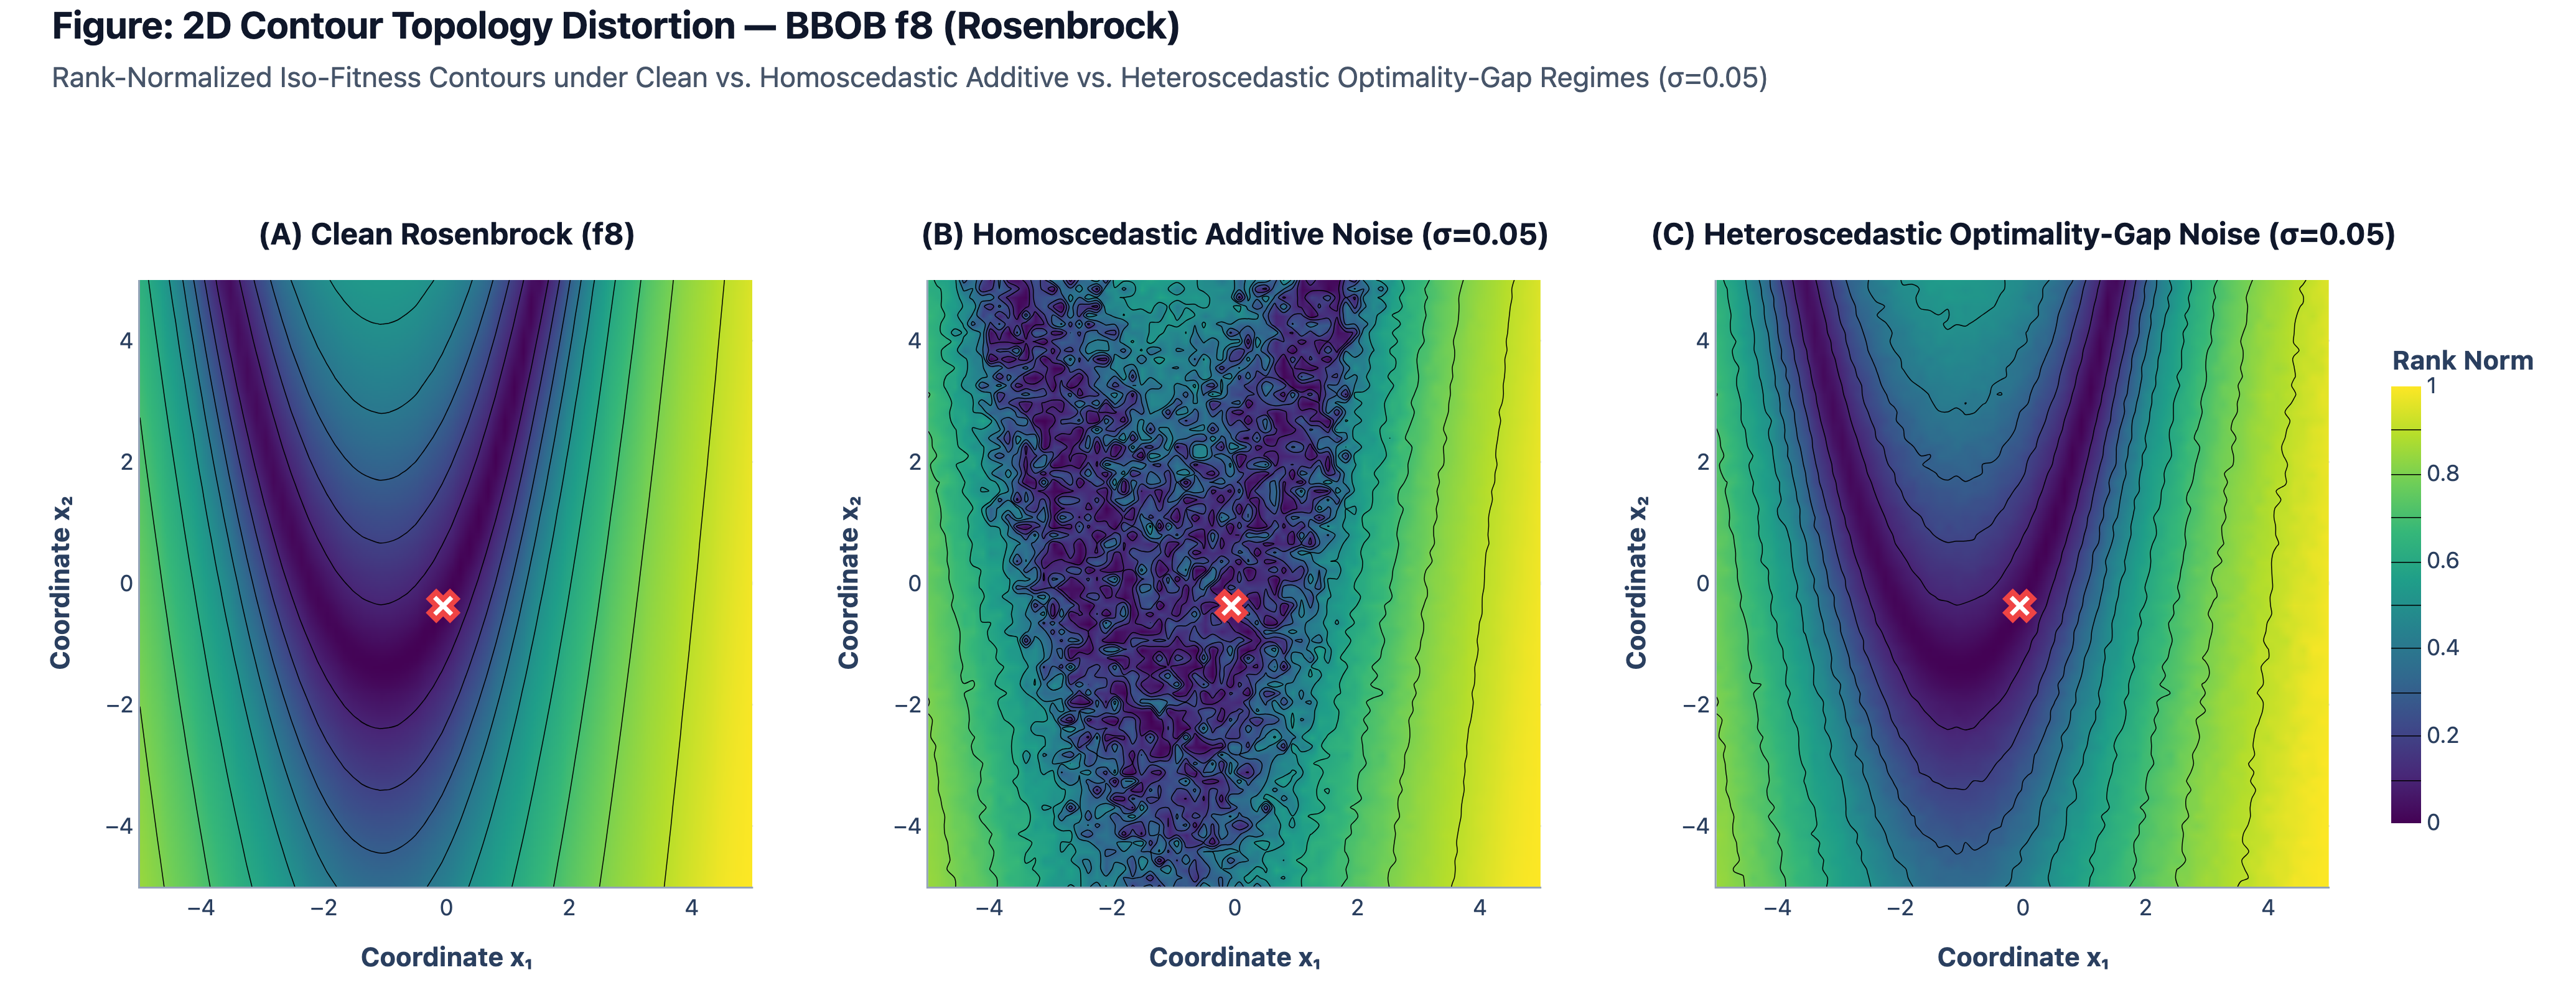
\includegraphics[width=\textwidth]
    {images/f8/figure_2d_noise_topology.png}

    \caption{Comparison of the clean, homoscedastic, and heteroscedastic
    evaluations of BBOB $f_8$ (Rosenbrock). The one-dimensional cross-section
    (top) and two-dimensional representation (bottom) show how the
    homoscedastic model applies a fixed calibrated perturbation scale across
    the problem, whereas the heteroscedastic model changes its standard
    deviation according to the clean optimality gap. The underlying clean
    objective remains unchanged in both stochastic formulations.}

    \label{fig:f8_noise_distortion}
\end{figure}

The second example is BBOB $f_{21}$, the Gallagher 101-peaks function. In
contrast to the narrow curved valley of $f_8$, this function contains many
local structures and provides a multimodal example in which stochastic
variation can alter the observed ranking of candidate points.

For the homoscedastic formulation, the same calibrated standard deviation is
used throughout the complete search space. The absolute perturbation scale
therefore remains fixed across regions with different objective errors.

For the heteroscedastic formulation, the perturbation scale is determined by
the clean objective gap at each queried point. The amount of stochastic
variation therefore changes across the function according to the remaining
objective error.

\begin{figure}[htbp]
    \centering

    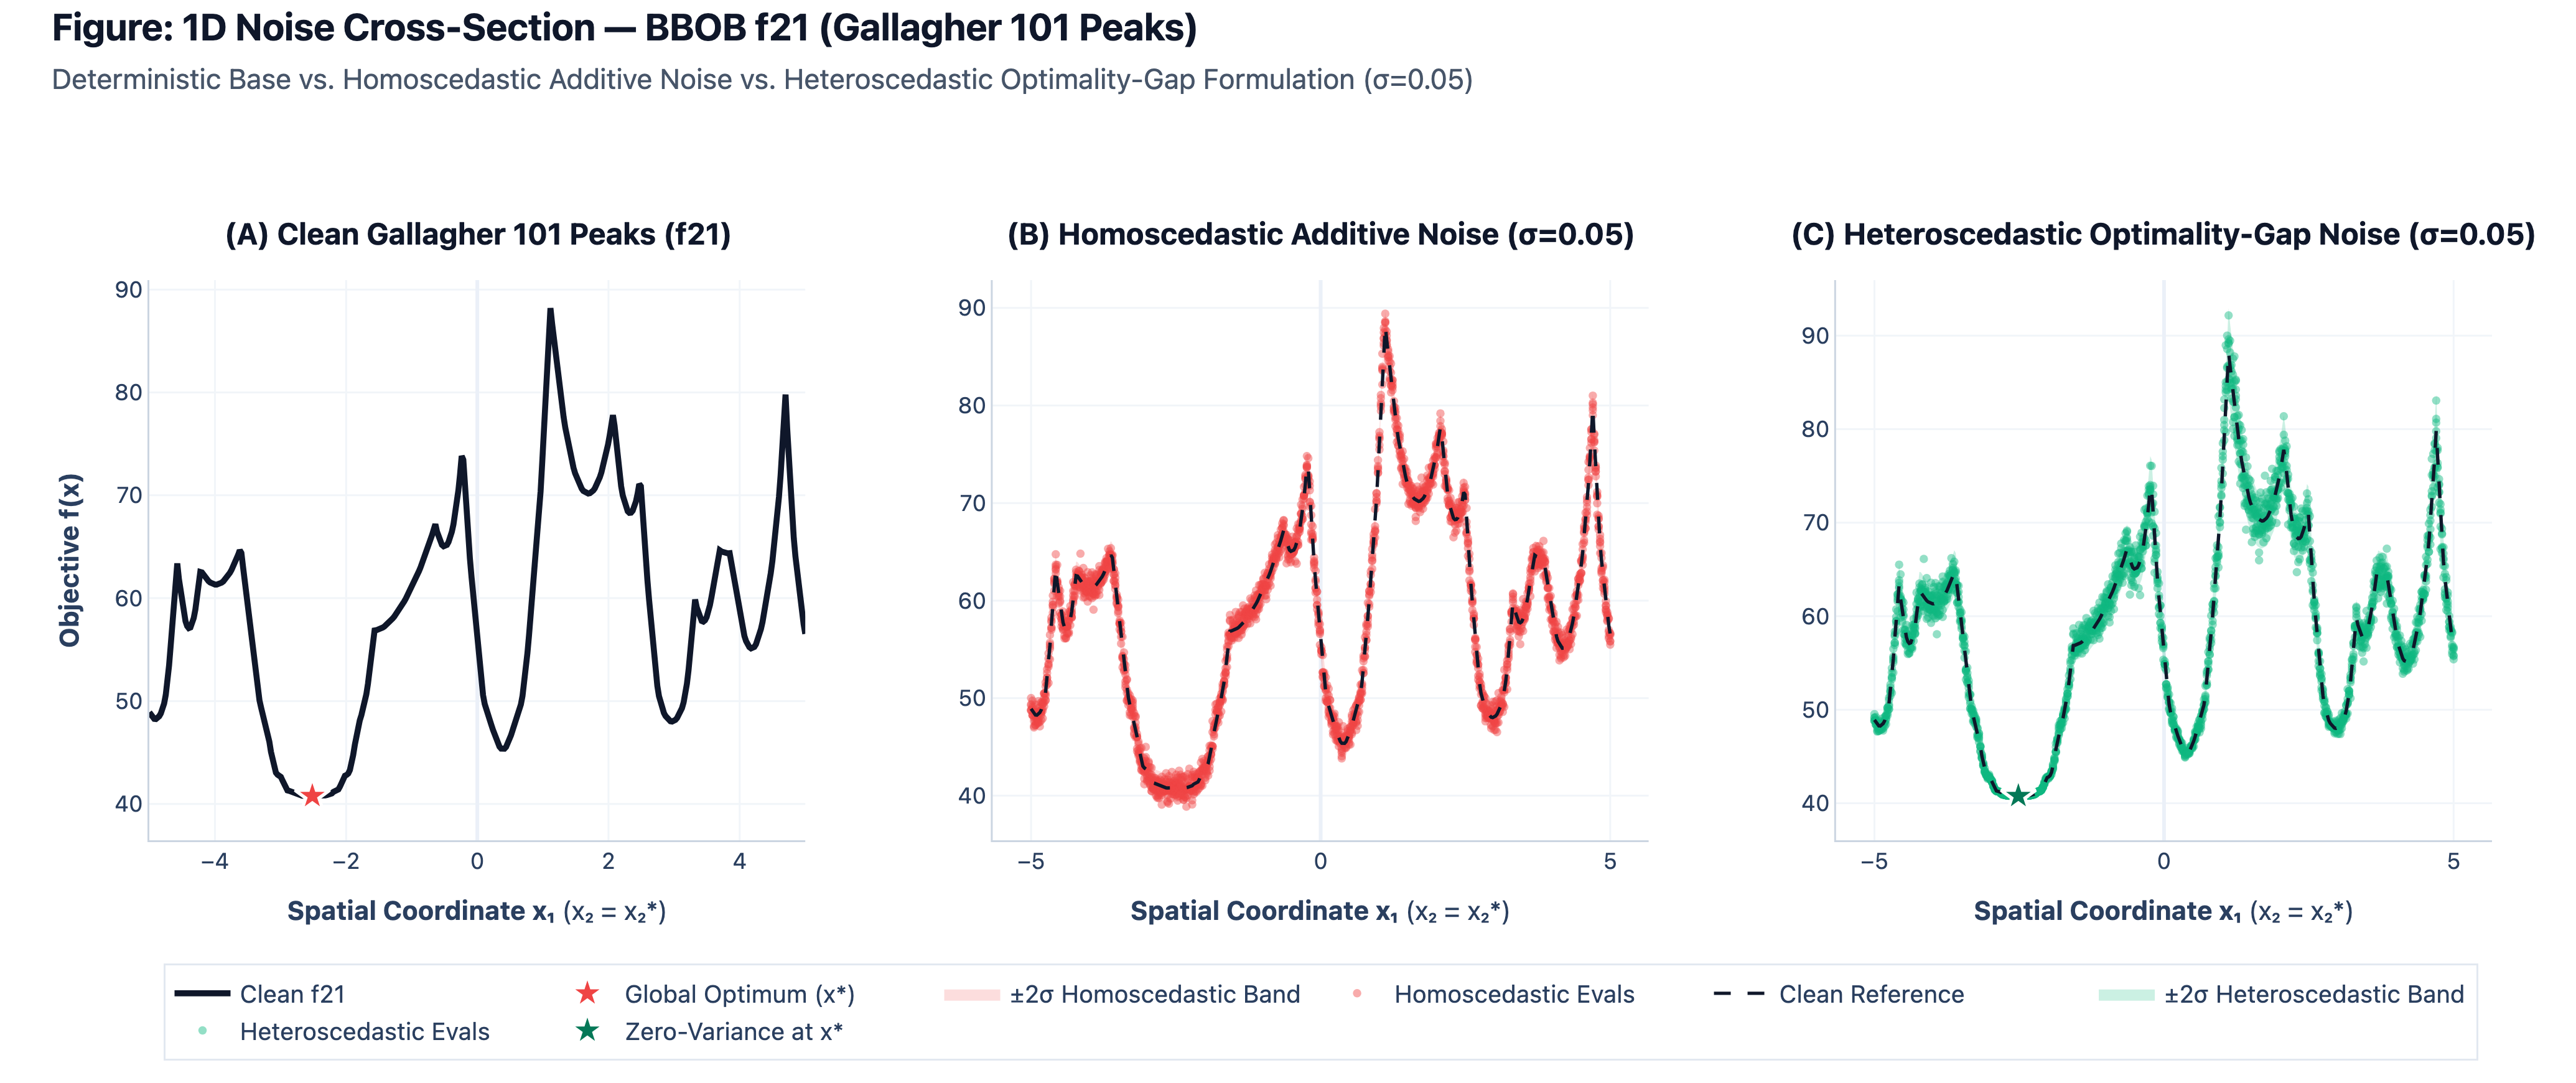
\includegraphics[width=\textwidth]
    {images/f21/figure_1d_noise_cross_section.png}

    \vspace{0.4cm}

    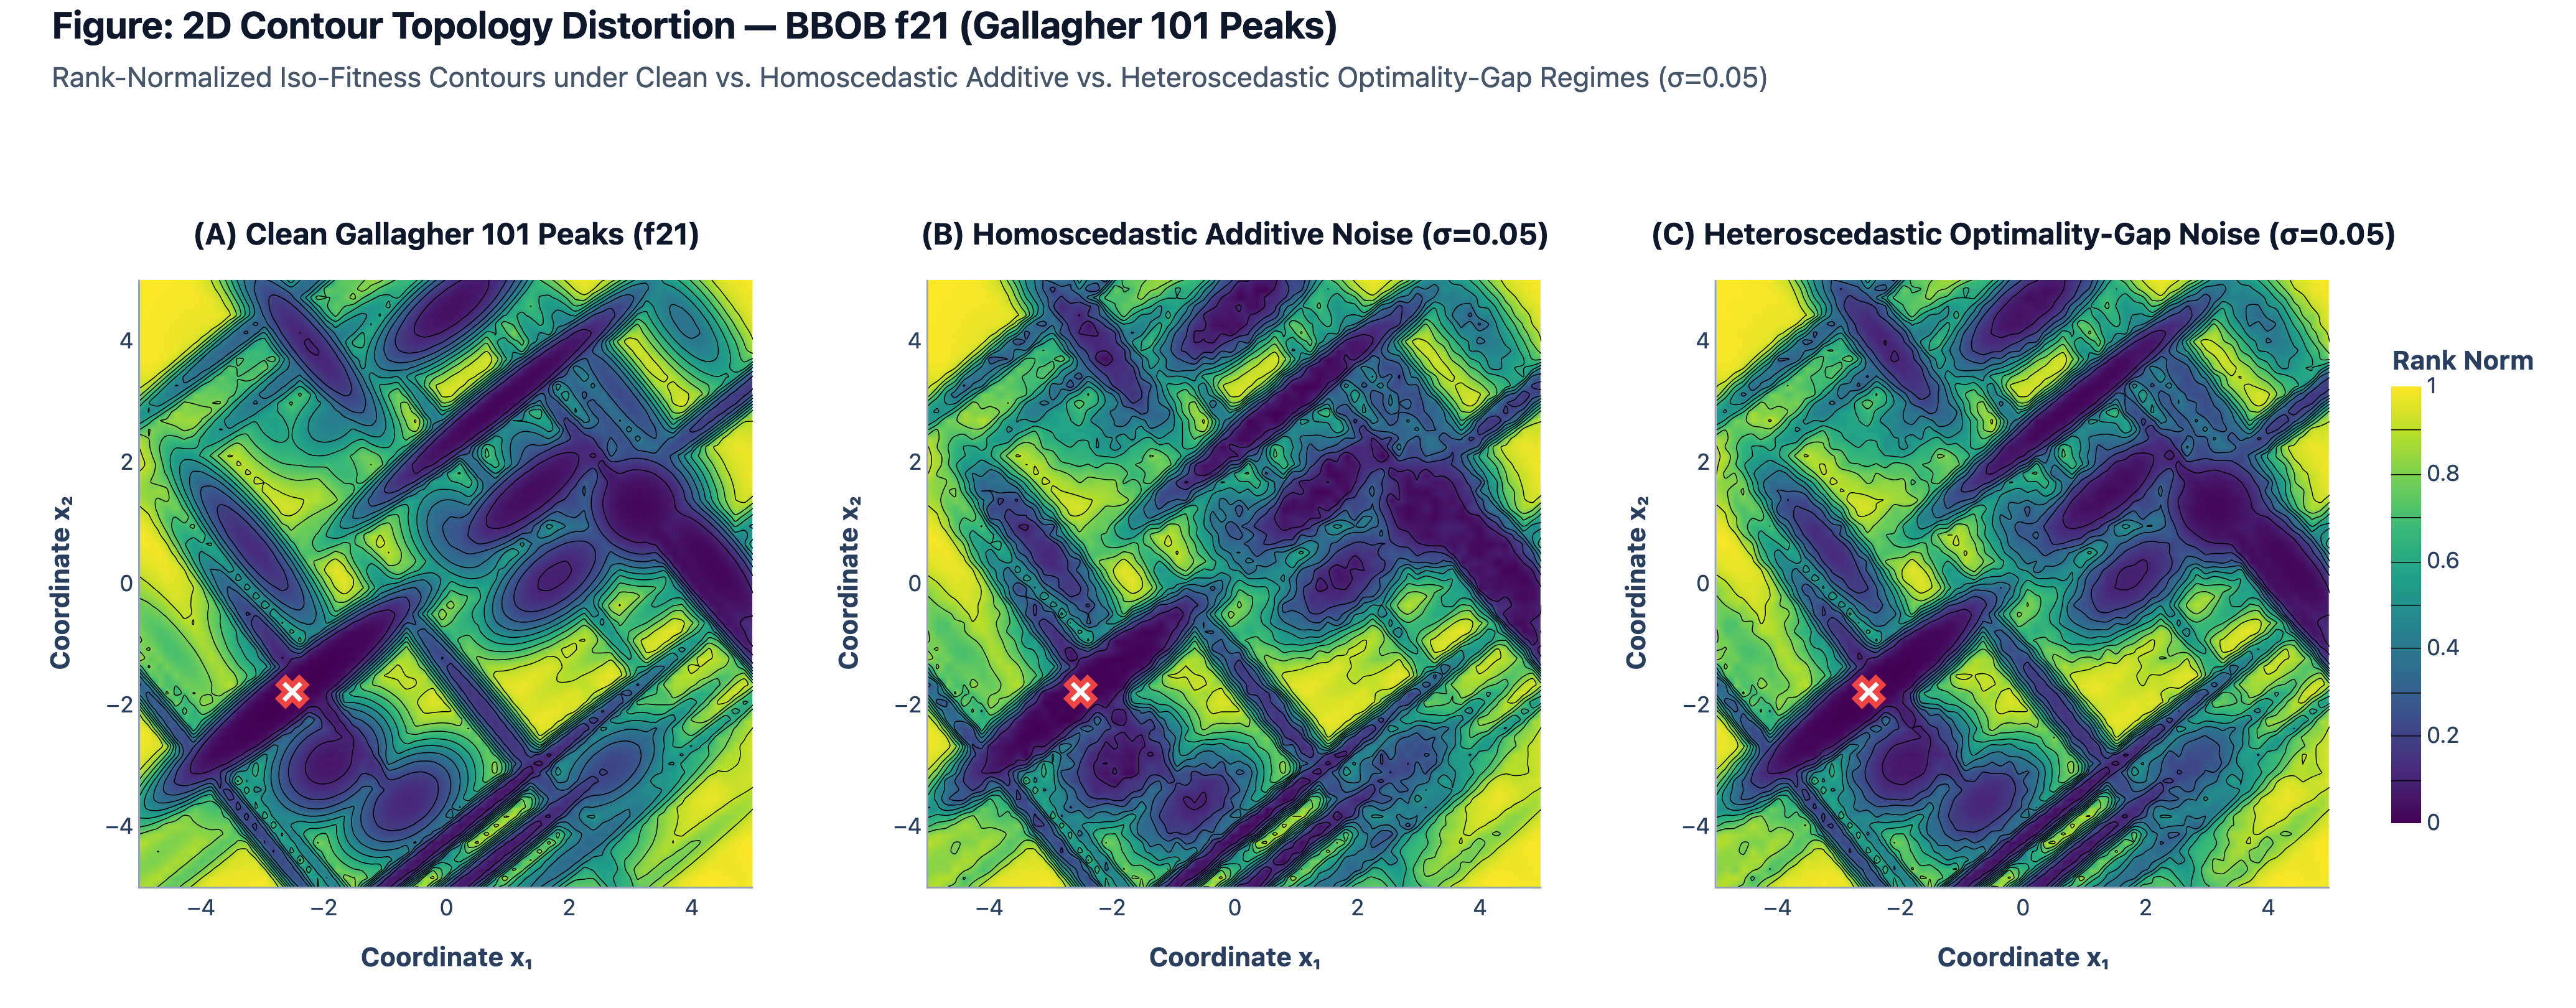
\includegraphics[width=\textwidth]
    {images/f21/figure_2d_noise_topology.png}

    \caption{Comparison of the clean, homoscedastic, and heteroscedastic
    evaluations of BBOB $f_{21}$ (Gallagher 101-peaks). The one-dimensional
    cross-section (top) and two-dimensional representation (bottom) show the
    clean function together with the fixed-scale homoscedastic perturbation
    and the optimality-gap-dependent heteroscedastic perturbation. The
    heteroscedastic formulation changes its stochastic scale according to the
    remaining clean objective error while leaving the underlying benchmark
    function unchanged.}

    \label{fig:f21_noise_distortion}
\end{figure}

The comparison does not imply that the homoscedastic formulation is generally
incorrect. The two models represent different assumptions about stochastic
fitness. The homoscedastic formulation assumes a constant absolute noise scale
within a calibrated problem. The heteroscedastic formulation assumes that the
magnitude of the stochastic perturbation changes with the remaining objective
error.

The heteroscedastic formulation is selected for the stochastic experiments in
this thesis because the intended experimental setup requires the reliability
of observed fitness values to change with optimization progress. It provides a
controlled stochastic model in which this dependency is explicitly defined
through the clean optimality gap.

The study does not assume that this formulation represents every possible
real-world source of noise. It defines the stochastic evaluation environment
under which the generated algorithms are synthesized and evaluated.


%==============================================================================
\section{LLM-Based Algorithm Synthesis}
\label{sec:llm_algorithm_synthesis}
%==============================================================================

The LLaMEA synthesis stage shown in
Figure~\ref{fig:methodology_architecture} operates on a continuous black-box
optimization task, the evaluation interface defined in the previous section,
and a prompt configuration defining the programming contract available to the
generated algorithm.

The generated algorithm is represented as a Python class following the
interface used by LLaMEA. Rather than producing one numerical solution
directly, the model produces a complete optimization procedure. This procedure
can contain its own initialization mechanism, population management,
candidate-generation operators, parameter updates, internal state, and
stopping logic.

The object being evolved is therefore not a solution vector but an executable
optimization algorithm. The LLM can change the structure of the search
procedure itself, including how candidate solutions are generated, how
previous observations are used, and how the search behavior changes during
execution.

This differs from conventional evolutionary optimization, where evolutionary
variation is typically applied directly to numerical solution
representations. In the present setting, the LLM performs variation at the
program level. The surrounding synthesis framework then determines whether
the generated program is valid and whether its observed optimization behavior
is sufficient for it to be retained.

At the system level, the synthesis framework provides the interface between
the language model, generated program, and evaluation environment. The LLM
produces source code from the current prompt and synthesis context. The
framework extracts this source, validates the required program contract,
executes the candidate in isolation, evaluates the returned result, and
converts the result into evolutionary feedback.

Once a candidate has passed validation, the synthesis controller treats the
generated optimizer as a black-box component. The optimizer receives the
supplied problem interface and an evaluation budget and is responsible for
constructing its own search procedure using only the information available
through that interface.

Figure~\ref{fig:llamea_synthesis_overview} shows the internal operation of the
synthesis stage. Starting from the optimization task and current synthesis
context, the LLM generates a candidate algorithm. The program is extracted
and validated before execution. During execution, the optimizer interacts with
the configured clean or stochastic objective interface.

After execution terminates, the returned solution is evaluated using the clean
objective by the outer framework. This algorithm-level diagnostic is used for
parent--child comparison and is also incorporated into the synthesis context
used for subsequent generations.

\begin{figure}[htbp]
    \centering
    \resizebox{!}{0.9\textheight}{%
        \begin{tikzpicture}[
    font=\footnotesize,
    >=Stealth,
    ioNode/.style={
        rectangle,
        draw=black!80,
        fill=yellow!15,
        text width=12.2cm,
        align=center,
        rounded corners=4pt,
        inner sep=7pt,
        thick
    },
    processNode/.style={
        rectangle,
        draw=black!80,
        fill=blue!5,
        text width=7.2cm,
        align=center,
        rounded corners=4pt,
        inner sep=6pt,
        thick,
        minimum height=1.2cm
    },
    evalNode/.style={
        processNode,
        fill=blue!10
    },
    selectionNode/.style={
        rectangle,
        draw=black!80,
        fill=purple!10,
        text width=12.2cm,
        align=center,
        rounded corners=4pt,
        inner sep=7pt,
        thick,
        minimum height=1.3cm
    },
    decision/.style={
        diamond,
        draw=black!80,
        fill=gray!15,
        thick,
        aspect=2.8,
        inner sep=3pt,
        align=center,
        font=\scriptsize,
        minimum width=5.6cm
    },
    outNode/.style={
        rectangle,
        draw=black!80,
        fill=green!15,
        text width=12.2cm,
        align=center,
        rounded corners=4pt,
        inner sep=7pt,
        thick,
        font=\footnotesize\bfseries
    },
    arrow/.style={
        ->,
        >=Stealth,
        thick,
        draw=black!75
    },
    fbArrow/.style={
        ->,
        >=Stealth,
        thick,
        draw=purple!80!black
    },
    elblB/.style={
        font=\scriptsize\bfseries,
        fill=white,
        inner sep=2pt,
        rounded corners=1pt
    }
]

    %----------------------------------------------------------------------
    % 1. Input Interface
    %----------------------------------------------------------------------
    \node[ioNode] (inputs) {
        \textbf{LLaMEA Synthesis Input}\\[2pt]
        \scriptsize Target Problem $(f_p, D, \sigma)$ \quad $\bullet$ \quad
        Active Prompt Scaffold $\mathcal{P}_{i,j}$ \quad $\bullet$ \quad
        Synthesis Budget $B_{\text{synth}} = 1{,}000$
    };

    %----------------------------------------------------------------------
    % 2. Reflective Context Assembly
    %----------------------------------------------------------------------
    \node[
        processNode,
        below=0.75cm of inputs
    ] (context) {
        \textbf{Reflective Context Assembly}\\[2pt]
        \scriptsize Compiles $\mathcal{C}_g = \{\mathcal{P}_{i,j}, \mathcal{A}_{\text{parent}}, \mathcal{T}_{\text{feedback}}, \mathcal{I}_{\text{directive}}\}$
    };

    %----------------------------------------------------------------------
    % 3. LLM Candidate Mutation
    %----------------------------------------------------------------------
    \node[
        processNode,
        below=0.7cm of context
    ] (generation) {
        \textbf{LLM Candidate Mutation}\\[2pt]
        \scriptsize Synthesizes executable optimization heuristic script $\mathcal{A}_{\text{child}}$
    };

    %----------------------------------------------------------------------
    % 4. AST Validation and Syntax Check
    %----------------------------------------------------------------------
    \node[
        processNode,
        below=0.7cm of generation
    ] (validation) {
        \textbf{AST Verification \& Parsing}\\[2pt]
        \scriptsize Validates imports, parses syntax tree, and extracts candidate class
    };

    %----------------------------------------------------------------------
    % 5. Sandboxed Runtime Execution (Single Execution Run)
    %----------------------------------------------------------------------
    \node[
        evalNode,
        below=0.7cm of validation
    ] (execution) {
        \textbf{Isolated Sandboxed Execution (Noisy Surface)}\\[2pt]
        \scriptsize Runs $\mathcal{A}_{\text{child}}$ on corrupted fitness feedback $f_{\text{noisy}}(x_k)$ ($T_{\text{max}} = 30.0\,\text{s}$)\\
        \scriptsize Returns candidate solution tuple: $(\mathbf{x}^*, y_{\text{raw}})$
    };

    %----------------------------------------------------------------------
    % 6. Ground-Truth Oracle Scoring (Evaluation on Clean Function)
    %----------------------------------------------------------------------
    \node[
        evalNode,
        fill=green!8,
        draw=green!55!black,
        below=0.75cm of execution
    ] (cleanOracle) {
        \textbf{Clean Ground-Truth Oracle Evaluation}\\[2pt]
        \scriptsize Discards noisy $y_{\text{raw}}$ and evaluates best coordinate on true objective:\\
        $y_{\text{clean}} = f_{\text{clean}}(\mathbf{x}^*)$ \quad $\implies$ \quad \\
        Optimality Gap: $\Delta y = |y_{\text{clean}} - f^*|$
    };

    %----------------------------------------------------------------------
    % 7. Selection, Resampling, and Context Update
    %----------------------------------------------------------------------
    \node[
        selectionNode,
        below=0.75cm of cleanOracle
    ] (selection) {
        \textbf{Parent--Child Comparison \& Incumbent Update}\\[2pt]
        \scriptsize Assigns selection fitness $\mathcal{F}(\mathcal{A}_{\text{child}}) = -\Delta y$, updates parent baseline $\bar{\mathcal{F}}_{\text{parent}}$,\\
        and appends diagnostic feedback buffer $\mathcal{T}_{\text{feedback}}$
    };

    %----------------------------------------------------------------------
    % 8. Termination Check
    %----------------------------------------------------------------------
    \node[
        decision,
        below=0.75cm of selection
    ] (termination) {
        \textbf{Generational Budget Reached?} ($g = G$)
    };

    %----------------------------------------------------------------------
    % 9. Final Terminal Output
    %----------------------------------------------------------------------
    \node[
        outNode,
        below=0.75cm of termination
    ] (output) {
        \textbf{Synthesized Champion Heuristic ($\mathcal{A}^*$)}\\[2pt]
        \scriptsize Validated Python optimizer class script and generational synthesis telemetry
    };

    %----------------------------------------------------------------------
    % Background Container Enclosure
    %----------------------------------------------------------------------
    \begin{scope}[on background layer]
        \node[
            draw=gray!50,
            dashed,
            fill=gray!3,
            rounded corners=8pt,
            inner sep=12pt,
            fit=(context) (generation) (validation) (execution) (cleanOracle) (selection),
            label={[font=\bfseries\scriptsize, text=gray!70!black]above:Iterative LLaMEA Evolutionary Engine}
        ] (loopGroup) {};
    \end{scope}

    %----------------------------------------------------------------------
    % Pipeline Forward Connectors
    %----------------------------------------------------------------------
    \draw[arrow] (inputs) -- (context);
    \draw[arrow] (context) -- (generation);
    \draw[arrow] (generation) -- node[elblB, right=2pt] {$\mathcal{A}_{\text{child}}$ Script} (validation);
    \draw[arrow] (validation) -- (execution);
    \draw[arrow] (execution) -- node[elblB, right=2pt] {Terminal Result $(\mathbf{x}^*, y_{\text{raw}})$} (cleanOracle);
    \draw[arrow] (cleanOracle) -- node[elblB, right=2pt] {True Error $\Delta y$} (selection);
    \draw[arrow] (selection) -- (termination);
    \draw[arrow] (termination) -- node[elblB, right=2pt] {Yes} (output);

    % Outer Loop Feedback (Routes cleanly on the outside left channel)
    \draw[fbArrow] (termination.west) -- ++(-3.8,0)
        node[elblB, pos=0.5, above, text=purple!80!black] {No: Next Generation ($g \gets g+1$)}
        |- (context.west);

\end{tikzpicture}
    }

    \caption{Detailed view of the LLaMEA-based algorithm synthesis process
    used in this thesis. The LLM generates candidate optimization heuristics,
    which are extracted, validated, and executed through the configured
    objective interface. The generated optimizer receives only the
    information exposed by that interface. After execution, the outer
    synthesis framework evaluates the returned solution using the clean
    objective, compares the child with the current incumbent, and updates the
    synthesis context for the following generation.}

    \label{fig:llamea_synthesis_overview}
\end{figure}


%------------------------------------------------------------------------------
\subsection{Synthesis Context}
\label{subsec:synthesis_context}
%------------------------------------------------------------------------------

The synthesis context contains the information required by the model to
generate or modify an algorithm. In the elitist $(1+1)$ setting, the context
can include the task description, information about previously generated
algorithms, the current incumbent, and feedback obtained from earlier
evaluations \cite{LLaMEA2024}.

Conceptually, the synthesis context at generation $g$ can be written as

\begin{equation}
\mathcal{C}_g
=
\{
\mathcal{P}_{\mathrm{task}},
\mathcal{H}_{1:g-1},
\mathcal{A}_{\mathrm{inc}},
\mathcal{F}_{\mathrm{prompt}}
\}.
\label{eq:synthesis_context}
\end{equation}

Here, $\mathcal{P}_{\mathrm{task}}$ represents the optimization task,
$\mathcal{H}_{1:g-1}$ represents information retained from previous
generations, $\mathcal{A}_{\mathrm{inc}}$ denotes the current incumbent
algorithm, and $\mathcal{F}_{\mathrm{prompt}}$ contains the instructions
defined by the selected prompt configuration.

The synthesis history can contain information about previous candidate
algorithms, their observed performance, and execution failures. This allows
the model to modify previously generated approaches rather than generating
every candidate independently.

The LLM uses this context to generate a new candidate. The model can modify an
existing algorithm or produce a substantially different search procedure.
Changes can therefore affect the complete search strategy rather than only
individual numerical parameters. A candidate can, for example, introduce a
different population-update mechanism, change the balance between exploration
and exploitation, adapt parameters during execution, or change how candidate
solutions are generated.

The generated response can contain explanatory text in addition to Python
source code. The implementation therefore extracts the candidate source before
execution. The resulting program is passed to the validation stage rather
than being executed directly from the raw model response.

The first valid candidate establishes the initial incumbent of the synthesis
run. It is generated using the same task, prompt configuration, and program
interface as subsequent candidates. Once this candidate has been executed,
its clean diagnostic evaluation establishes the reference against which later
children are compared.

The synthesis run terminates according to the configured stopping criteria.
These criteria include the maximum permitted synthesis generations and/or the
synthesis evaluation budget used by the experimental configuration. Their
exact values are reported in Chapter~\ref{chap:experiments}.

At termination, the current incumbent is retained as the synthesized optimizer
produced by that run. The retained algorithm is subsequently passed to the
independent benchmark stage.


%------------------------------------------------------------------------------
\subsection{Candidate Validation and Execution}
\label{subsec:candidate_validation_execution}
%------------------------------------------------------------------------------

The candidate validation and execution stage defines the boundary between the
generated program and the evaluation environment.

The process first identifies the Python source contained in the generated
response and prepares it for execution. Since language-model responses can
contain explanations, Markdown formatting, or other text in addition to the
requested program, the extraction step creates a clear boundary between model
output and executable candidate code.

The resulting program is checked structurally using Abstract Syntax Tree
(AST) analysis. This validation stage detects malformed or disallowed code
before it reaches the execution environment.

The implementation permits the numerical functionality required for the
optimization task while preventing generated code from delegating the search
to prohibited external optimization routines or interacting directly with the
surrounding operating system.

The purpose of the validator is not to restrict the model to a particular
optimization strategy. Instead, it ensures that different generated algorithms
are evaluated through the same interface and within the same execution
constraints.

A candidate must provide the required optimizer class, constructor, callable
interface, and return value. The source must also be syntactically valid.
Imports or calls that delegate the optimization task to prohibited pre-built
optimization solvers are rejected.

The main requirements are summarized in
Table~\ref{tab:validation_requirements}.

\begin{table}[htbp]
    \centering
    \caption{Structural and execution requirements imposed on generated
    optimization algorithms.}
    \label{tab:validation_requirements}

    \begin{tabular}{|p{0.30\textwidth}|p{0.60\textwidth}|}
        \hline
        \textbf{Requirement} & \textbf{Validation condition} \\
        \hline

        Python source &
        The extracted candidate must be syntactically valid Python. \\
        \hline

        Optimizer class &
        The candidate must provide the required optimizer class. \\
        \hline

        Constructor &
        \texttt{\_\_init\_\_(self)} must not require additional arguments. \\
        \hline

        Callable interface &
        The optimizer must provide
        \texttt{\_\_call\_\_(self, problem, budget)}. \\
        \hline

        Return value &
        The optimizer must return
        \texttt{(best\_x, best\_y)}. \\
        \hline

        Optimization logic &
        The search procedure must be implemented directly rather than
        delegated to prohibited external optimization solvers. \\
        \hline

        Variable validity &
        Variables must be defined before use. \\
        \hline

        Execution boundary &
        The candidate must operate through the supplied objective interface
        and remain within the provided search bounds and evaluation budget. \\
        \hline
    \end{tabular}
\end{table}

The table describes the observable contract of the validator rather than its
source-code implementation. The exact AST rules used to identify prohibited
imports, calls, and structural violations are implementation details and are
applied consistently to every generated candidate.

After validation, the candidate is compiled and executed in an isolated
worker process. Isolation prevents variables or process state created by one
candidate from affecting the surrounding synthesis process. It also allows a
generated algorithm to be terminated independently if it does not complete
within the permitted execution time.

The generated optimizer interacts with the optimization problem only through
the objective-function interface provided to it. Under stochastic evaluation,
it does not directly access the analytical benchmark function, the known
optimum, or the clean diagnostic objective.

From the perspective of the generated algorithm, the objective is therefore
an externally supplied function that can be queried at candidate points. The
optimizer must construct its search strategy from the values returned by these
queries.

The worker process provides an execution boundary between candidate evaluation and the rest of the synthesis framework. Candidate execution is subject to a maximum runtime, and runtime failures are recorded so that they do not normally terminate the complete synthesis process. Where appropriate, diagnostic information is included in the context supplied to later generations, allowing the model to use execution feedback when revising a program, consistent with the feedback-driven design of LLaMEA \cite{LLaMEA2024}.

Let $T_{\mathrm{exec}}$ denote the maximum permitted execution time for one candidate. If execution exceeds this limit, the candidate is classified as a timeout. The execution time limit is treated as an implementation constraint rather than as an optimization objective; its experimental value is reported in Chapter~\ref{chap:experiments}.

Generated algorithms may fail because of invalid numerical operations, incompatible array dimensions, incorrect use of the objective interface, undefined variables, or other implementation errors. These failures are captured during candidate evaluation and recorded with diagnostic information. They are handled as candidate failures rather than being allowed to terminate the complete synthesis process.

For the standard return format \texttt{(best\_x, best\_y)}, the evaluation environment checks that \texttt{best\_x} has the expected dimension and lies within the problem bounds, allowing a small numerical tolerance. Non-finite coordinates fail this bounds check. The environment then evaluates \texttt{best\_x} on the clean objective and rejects a non-finite objective value.

Let $B$ denote the configured objective-evaluation budget and let $N_{\mathrm{eval}}$ denote the number of objective evaluations. The intended protocol is

\begin{equation}
N_{\mathrm{eval}} \leq B.
\label{eq:evaluation_budget}
\end{equation}

Each actual evaluation through \texttt{problem(x)} counts, including repeated evaluations of the same point. The generated optimizer is instructed to maintain an internal evaluation counter and stop objective queries before exceeding the configured budget. The common prompt example performs an initial evaluation and sets its counter to one before beginning further search.

This inequality is an intended protocol, not a strict runtime guarantee in the current implementation. Although the BBOB wrapper can enforce a hard cap when a budget is set on the problem, the synthesis path does not currently set that cap. The executor records the observed evaluation count and warns about substantial overruns, but does not reject every over-budget candidate.

For the standard return format, \texttt{best\_x} is the coordinate vector selected by the generated optimizer, and \texttt{best\_y} is the objective value it reports for that vector. Under stochastic evaluation, \texttt{best\_y} may reflect a noisy observation. The outer synthesis framework therefore uses a clean reevaluation of \texttt{best\_x} as the algorithm-level selection criterion, following the procedure described in Section~\ref{subsec:deterministic_stochastic}. For a scalar-only return, no \texttt{best\_x} is available for clean reevaluation, so the framework uses the returned scalar value instead.


%==============================================================================
\section{Selection and Feedback}
\label{sec:candidate_selection}
%==============================================================================

Once a generated candidate has been executed, its result is returned to the
outer evolutionary controller. The controller uses the clean diagnostic
quality of the returned solution to compare the candidate with the current
incumbent.

This is a deliberate part of the methodology rather than an information
channel available to the generated optimizer.

The distinction corresponds to two nested levels of optimization. The inner
level is the search performed by the generated optimization program. Under
stochastic conditions, this optimizer receives only noisy objective
observations and does not know the clean optimum or clean objective values.

The outer level is the LLaMEA algorithm-design process. Its task is not to
optimize a solution vector directly, but to compare complete generated
optimization algorithms. The clean diagnostic objective is therefore used at
this outer level so that parent and child algorithms can be compared according
to the quality of the solutions they produce.

The outer synthesis process consequently has access to information that is
intentionally unavailable to the generated optimizer. The generated algorithm
must still discover its returned solution entirely through the objective
interface supplied during execution.


%------------------------------------------------------------------------------
\subsection{Parent--Child Comparison}
\label{subsec:parent_child_comparison}
%------------------------------------------------------------------------------

For a parent algorithm $\mathcal{A}_{\mathrm{parent}}$ and a child algorithm
$\mathcal{A}_{\mathrm{child}}$, let

\begin{equation}
\Delta f_{\mathrm{parent}}
=
\Delta f(x_{\mathrm{parent}})
\end{equation}

and

\begin{equation}
\Delta f_{\mathrm{child}}
=
\Delta f(x_{\mathrm{child}})
\end{equation}

denote the clean optimality gaps of their returned solutions.

The parent corresponds to the currently retained algorithm, while the child
is the newly generated algorithm produced from the current synthesis context.
The synthesis process uses one parent and one offspring with elitist
selection, corresponding to a $(1+1)$ evolutionary structure.

Each generated child is executed once by the evaluation framework. During
this execution, the optimizer interacts with the configured objective
interface. Under stochastic conditions, these observations follow the
stochastic model defined in
Section~\ref{sec:problem_evaluation_setup}.

After the execution has finished, the returned solution is evaluated using the
clean objective. The corresponding clean error is

\begin{equation}
\Delta f(x_{\mathrm{best}})
=
\left|
f_{\mathrm{clean}}(x_{\mathrm{best}}) - f^*
\right|.
\label{eq:clean_optimality_gap_selection}
\end{equation}

Here, $f^*$ is the known global minimum value of the clean benchmark
objective, as defined in Equation~\ref{eq:true_optimum}. It is available to
the outer evaluator but not to the generated optimizer during its search.

The error is converted into the fitness score used by LLaMEA,

\begin{equation}
S = -\Delta f.
\label{eq:synthesis_fitness_score}
\end{equation}

The minus sign is used because the outer controller selects larger fitness
scores, whereas a smaller clean error is better.

Smaller clean optimality gaps therefore correspond to larger fitness scores.
A candidate with zero clean error receives the maximum possible score of
zero.

The child replaces the current incumbent when its clean optimality gap is
strictly smaller than the clean optimality gap previously recorded for the
parent:

\begin{equation}
\Delta f_{\mathrm{child}}
<
\Delta f_{\mathrm{parent}}.
\label{eq:child_replacement_condition}
\end{equation}

If this condition is not satisfied, the current parent remains the incumbent.

The parent is not re-executed before the comparison. Its previously recorded
clean diagnostic score remains the reference used for elitist selection.

Each generated child is executed once during synthesis. Its returned solution
therefore still depends on the search trajectory produced during that
particular execution. Here, the search trajectory means the sequence of
points evaluated by the generated optimizer and the decisions it makes from
the observed objective values.

Under stochastic evaluation, a different sequence of stochastic observations
could cause the same generated algorithm to return a different solution. The
clean post-execution evaluation removes stochasticity from the measurement of
the returned point, but it does not remove stochasticity from the trajectory
that produced that point.

Robustness across repeated random seeds is therefore assessed during the
independent benchmark evaluation rather than by repeatedly executing every
candidate during synthesis.

%------------------------------------------------------------------------------
\subsection{Feedback and Context Update}
\label{subsec:feedback_update}
%------------------------------------------------------------------------------

After the parent--child comparison, information from the candidate evaluation
is added to the synthesis context used in the following generation.

This feedback is not an additional selection criterion. Whether the child
replaces the parent remains determined by the clean algorithm-level score
described above.

The role of the feedback is instead to communicate what occurred during the
candidate evaluation so that the LLM can use this information when generating
the next candidate.

The deliberate inner/outer information separation also applies to this
feedback. The generated optimizer does not observe the clean diagnostic value
while it is executing. Once execution has finished, however, the outer
synthesis framework can include the resulting clean algorithm-level error in
the evolutionary feedback supplied to the LLM.

The LLM therefore receives information about how successful the previously
generated optimizer was, while the optimizer itself still had to perform its
search using only the configured objective observations.

For a candidate that executes successfully, the evaluator reports its final
objective error. A typical result message is:

\begin{verbatim}
[RESULT]

The generated algorithm executed successfully.

Final objective error:

0.0012

Use this result together with the previous algorithm history when
designing the next candidate.
\end{verbatim}

When the candidate is evaluated under a stochastic objective, the feedback
can additionally make the stochastic setting explicit:

\begin{verbatim}
[RESULT]

The generated algorithm executed successfully on a stochastic objective.

Final objective error:

0.8420

The result indicates that the current search strategy may not have
handled the stochastic evaluations effectively.

Use the observed result and previous algorithm history to improve
the next candidate.
\end{verbatim}

The numerical error in these messages is obtained from the clean
post-execution diagnostic evaluation of the returned solution. It is
therefore an outer-loop algorithm-level performance signal rather than an
objective observation that was available to the generated optimizer during
its search.

The feedback does not prescribe which optimization algorithm the LLM should
generate next. It reports the observed result and leaves the next algorithmic
decision to the synthesis process.

Candidates that fail during execution are handled differently. Rather than
providing only a poor score, the evaluator reports the cause of the failure so
that a subsequent generated program can address it.

For example:

\begin{verbatim}
[RUNTIME ERROR]

The generated algorithm failed during execution.

Error:

ValueError: shapes (10, 2) and (3, 10) not aligned: 2 != 3

Relevant code:

  -> line   8:     arr = pop @ weights

Fix the cause of the failure in the next candidate.

Ensure that:

- array shapes and dimensions are valid;
- numerical operations are well-defined;
- all variables are initialized before use;
- the search stays within the provided bounds;
- every objective evaluation is counted;
- the total number of objective evaluations does not exceed the budget.

Problem context: BBOB-1, dim=3, bounds=[-5.0, 5.0].
\end{verbatim}

The message therefore gives the LLM information directly related to the
observed implementation problem. This can include invalid array dimensions,
undefined variables, numerical errors, violations of the search bounds, or
incorrect evaluation-budget handling.

The intention is not to explain the complete implementation to the model, but
to provide sufficient diagnostic information for a later candidate to correct
the observed failure.

For candidates evaluated under stochastic fitness, the runtime diagnostic can
be extended with the following context:

\begin{verbatim}
[NOISY PROBLEM CONTEXT]

The objective function is stochastic.

Ensure that optimization decisions are not based on invalid or
inconsistently stored objective values.

Keep any internal statistical estimates separate from the
objective value required by the optimizer interface.

Ensure that every call to problem(x) is counted against the
evaluation budget.
\end{verbatim}

This information is deliberately kept general. It does not require the LLM to
use a particular noise-handling technique, a fixed number of repeated
evaluations, or a predefined statistical estimator.

Such decisions remain part of the generated optimization algorithm.

Execution time is treated separately from ordinary runtime errors. If a
candidate exceeds the allowed execution time, the evaluator reports:

\begin{verbatim}
[TIMEOUT]

The generated algorithm exceeded the execution time limit.

Reduce unnecessary computation and ensure that the implementation
can complete within the available execution time and evaluation
budget.

Problem context: BBOB-1, dim=3, bounds=[-5.0, 5.0].
\end{verbatim}

The stochastic problem context can again be attached when the candidate was
evaluated under stochastic fitness.

A separate case occurs when several consecutive candidates fail. Without
additional intervention, the LLM may continue making minor modifications to
an unsuccessful implementation.

The implementation therefore tracks consecutive execution failures. Let
$K_{\mathrm{fail}}$ denote the configured failure threshold. Once the number
of consecutive failures reaches this threshold, meta-feedback is added to the
synthesis history:

\begin{verbatim}
[META-FEEDBACK]

The last several generated algorithms failed to execute correctly.

Try a substantially different search mechanism rather than making
only minor modifications to the previous approach.

Check the previous implementation for the source of the failure and
ensure that the new algorithm respects the objective interface,
search bounds, evaluation budget, and numerical constraints.
\end{verbatim}

After a successful candidate, the consecutive-failure counter is reset. The
activation of the meta-feedback therefore depends on the observed execution
sequence rather than on the candidate's optimization score.

In this implementation, meta-feedback is activated after
$K_{\mathrm{fail}} = \text{3}$ consecutive candidate failures.

The meta-feedback deliberately does not recommend a particular optimization
algorithm. This keeps the synthesis process separate from the external
benchmark algorithms used later during independent evaluation.

Taken together, the feedback messages provide information about what happened
to the previous candidate while leaving the evolutionary selection mechanism
unchanged. A successful candidate contributes its observed algorithm-level
performance, a failed candidate contributes diagnostic information about its
execution problem, and repeated failures can trigger a request for a
substantially different search mechanism.

This information is accumulated in the synthesis history
$\mathcal{H}_{1:g-1}$ introduced in
Equation~\ref{eq:synthesis_context}. At generation $g$, the relevant history
is supplied to the LLM together with the current task prompt.


%==============================================================================
\section{Prompt Design}
\label{sec:prompt_design}
%==============================================================================

The prompt sent to the LLM has three components: \texttt{TASK},
\texttt{EXAMPLE}, and \texttt{FORMAT}. They are assembled in this order:

\begin{verbatim}
TASK
EXAMPLE
FORMAT
\end{verbatim}

The \texttt{EXAMPLE} and \texttt{FORMAT} components remain fixed across
synthesis conditions. The \texttt{TASK} component is assembled for each
condition from a common task layout, one selected environment-information
block, and one selected strategy scaffold. Thus, the environment and strategy
variants form the variable content within \texttt{TASK}.

The environment-information design is organized hierarchically. At the first
level, a condition is either \textsc{Implicit} or \textsc{Explicit}.

In the \textsc{Implicit} condition, the prompt informs the model only that
repeated evaluations of the same point may differ. It does not explicitly
identify the evaluation environment as stochastic and does not describe the
source or magnitude of the variation.

The \textsc{Explicit} branch is divided into two settings. The
\textsc{Explicit--Clean} condition states directly that the objective is
deterministic. The \textsc{Explicit--Noisy} condition states directly that
the objective is stochastic and that repeated evaluations can differ because
of random variation.

Each of these three resulting environment-information conditions is combined
with one of four strategy scaffolds:

\begin{itemize}
    \item \textsc{Baseline},
    \item \textsc{Vectorization},
    \item \textsc{Guided},
    \item \textsc{Thinking}.
\end{itemize}

The design therefore contains four \textsc{Implicit} configurations, four
\textsc{Explicit--Clean} configurations, and four
\textsc{Explicit--Noisy} configurations, resulting in twelve prompt
conditions.

Figure~\ref{fig:prompt_architecture} summarizes the prompt architecture.

\begin{figure}[htbp]
    \centering

    \resizebox{\textwidth}{!}{%
        \begin{tikzpicture}[
    font=\footnotesize,
    >=Stealth,
    base/.style={
        rectangle, rounded corners=3pt, thick, align=center,
        inner sep=3.5pt
    },
    root/.style={
        base, draw=blue!75!black, fill=blue!10,
        text width=11.5cm, minimum height=0.7cm,
        font=\small\bfseries
    },
    fixedbox/.style={
        base, draw=blue!75!black, fill=blue!8,
        text width=3.5cm, minimum height=0.65cm,
        font=\scriptsize\bfseries
    },
    fixeditem/.style={
        base, draw=blue!50!black, fill=blue!2,
        text width=3.5cm, align=left, inner sep=3.5pt,
        font=\tiny
    },
    taskbox/.style={
        base, draw=orange!75!black, fill=orange!8,
        text width=8.5cm, minimum height=0.72cm,
        font=\scriptsize\bfseries
    },
    taskitem/.style={
        base, draw=orange!55!black, fill=orange!3,
        text width=8.0cm, minimum height=0.6cm,
        font=\scriptsize
    },
    modeparent/.style={
        base, rounded corners=3pt,
        text width=3.25cm, minimum height=0.8cm,
        font=\scriptsize\bfseries
    },
    subenv/.style={
        base, rounded corners=2pt,
        text width=1.45cm, minimum height=0.52cm,
        font=\scriptsize
    },
    stratbanner/.style={
        base, draw=purple!65!black, fill=purple!8,
        text width=7.9cm, minimum height=0.55cm,
        font=\scriptsize\bfseries
    },
    stratbox/.style={
        base, rounded corners=2pt,
        draw=purple!60!black, fill=purple!5,
        text width=1.75cm, minimum height=0.55cm,
        inner sep=2pt, font=\scriptsize
    },
    treearrow/.style={->, >=Stealth, thick, draw=black!70}
]

% The LLM request has invariant components and a condition-specific TASK.
\node[root] (root) {Prompt Assembly};

\node[fixedbox, below=0.9cm of root.south, xshift=-4.4cm] (fixed) {
    Invariant Components
};
\node[taskbox, below=0.9cm of root.south, xshift=3.8cm] (task) {
    \texttt{TASK} Prompt (assembled for each condition)
};

\draw[treearrow] (root.south) -- ++(0,-0.35) -| (fixed.north);
\draw[treearrow] (root.south) -- ++(0,-0.35) -| (task.north);

% Only EXAMPLE and FORMAT are invariant across synthesis conditions.
\node[fixeditem, below=0.8cm of fixed] (example) {
    \textbf{\texttt{EXAMPLE}}\\
    Common algorithm class, \texttt{\_\_init\_\_}, \texttt{\_\_call\_\_},
    bound extraction, budget tracker.
};
\node[fixeditem, below=0.55cm of example] (format) {
    \textbf{\texttt{FORMAT}}\\
    Uniform response schema, single block, return tuple
    $(\mathbf{x}^*, y_{\text{raw}})$, whitelist NumPy.
};
\draw[treearrow] (fixed.south) -- (example.north);
\draw[treearrow] (example.south) -- (format.north);

% The TASK prompt contains a shared layout and selected variable blocks.
\node[taskitem, below=0.65cm of task] (layout) {
    \textbf{Task Layout}\\
    Target identifier, dimension $D$, bounds $[-5,5]^D$, evaluation budget
    $B_{\text{synth}}$, and tags.
};
\node[taskitem, below=0.55cm of layout] (environment) {
    Select one environment-information block
};
\draw[treearrow] (task.south) -- (layout.north);
\draw[treearrow] (layout.south) -- (environment.north);

\node[
    modeparent, draw=yellow!65!black, fill=yellow!12,
    below=0.6cm of environment.south, xshift=-2.1cm
] (implicit) {
    \textbf{Implicit}\\[-1pt]
    \tiny Repeated evaluations may differ
};
\node[
    modeparent, draw=orange!75!black, fill=orange!12,
    below=0.6cm of environment.south, xshift=2.1cm
] (explicit) {
    \textbf{Explicit}\\[-1pt]
    \tiny Evaluation behavior is stated
};
\draw[treearrow] (environment.south) -- ++(0,-0.22) -| (implicit.north);
\draw[treearrow] (environment.south) -- ++(0,-0.22) -| (explicit.north);

\node[
    subenv, draw=green!60!black, fill=green!8,
    below=0.5cm of explicit.south, xshift=-0.9cm
] (clean) {Clean};
\node[
    subenv, draw=red!60!black, fill=red!8,
    below=0.5cm of explicit.south, xshift=0.9cm
] (noisy) {Noisy};
\draw[treearrow] (explicit.south) -- ++(0,-0.18) -| (clean.north);
\draw[treearrow] (explicit.south) -- ++(0,-0.18) -| (noisy.north);

\node[
    stratbanner,
    below=0.75cm of clean.south -| environment.south
] (scaffolds) {Select one strategy scaffold};
\draw[treearrow] (implicit.south) -- (implicit.south |- scaffolds.north);
\draw[treearrow] (clean.south) -- (clean.south |- scaffolds.north);
\draw[treearrow] (noisy.south) -- (noisy.south |- scaffolds.north);

\node[stratbox, below=0.45cm of scaffolds.south west,
      anchor=north west, xshift=0.08cm] (baseline) {Baseline};
\node[stratbox, right=0.15cm of baseline] (thinking) {Thinking};
\node[stratbox, right=0.15cm of thinking] (vectorization) {Vectorization};
\node[stratbox, right=0.15cm of vectorization] (guided) {Guided};
\draw[treearrow] (scaffolds.south -| baseline.north) -- (baseline.north);
\draw[treearrow] (scaffolds.south -| thinking.north) -- (thinking.north);
\draw[treearrow] (scaffolds.south -| vectorization.north) -- (vectorization.north);
\draw[treearrow] (scaffolds.south -| guided.north) -- (guided.north);

\node[taskitem, below=1.55cm of scaffolds.south] (combinations) {
    3 environment conditions $\times$ 4 scaffolds = 12 \texttt{TASK} variants
};

\end{tikzpicture}

    }

    \caption{Prompt composition used for synthesis. The \texttt{EXAMPLE} and
    \texttt{FORMAT} components are invariant. For each synthesis condition,
    the \texttt{TASK} prompt combines the common task layout with one selected
    environment-information block and one strategy scaffold. The environment
    choices are \textsc{Implicit}, \textsc{Explicit--Clean}, and
    \textsc{Explicit--Noisy}; the strategy choices are \textsc{Baseline},
    \textsc{Thinking}, \textsc{Vectorization}, and \textsc{Guided}. Their
    combinations produce twelve \texttt{TASK} variants, each assembled with
    the same \texttt{EXAMPLE} and \texttt{FORMAT}.}

    \label{fig:prompt_architecture}
\end{figure}


%..............................................................................
% FORMAT component
%..............................................................................

The common \texttt{FORMAT} component defines how the LLM must return the
generated algorithm. Its complete content is:

\begin{verbatim}
Respond with EXACTLY the following format -- no extra code blocks:

Feedback: <your reasoning and description of the algorithm>

Code:

```python

<your complete class and any required imports>

````

STRICT Rules -- violating any rule will cause execution failure:

* There must be exactly ONE `python ... ` block in your response.

* The class MUST be named exactly one word
  (e.g., class MyOptimizer:).

* **init**(self) MUST take NO extra arguments beyond self.

* **init**(self) MUST have a non-empty body
  (use pass if nothing to initialize).

* The class MUST have a **call**(self, problem, budget) method.

* **call** MUST return (best_x, float(best_y)) -- a tuple of the
  best search coordinates array and best scalar float value.

* Do NOT import or call scipy.optimize
  (e.g., scipy.optimize.minimize, differential_evolution, etc.).
  Pre-built solver wrappers are strictly banned.
  Write your search algorithm logic from scratch using NumPy.

* Every variable you use MUST be defined before use.
  Never reference undefined names.

* Do NOT store problem or budget in **init**.
  They are provided to **call** directly.

* Do NOT include if **name** == '**main**': blocks.
\end{verbatim}

The output requirements are common to every generated algorithm. In
particular, the return value always contains \texttt{best\_x} and
\texttt{best\_y}. These values form part of the common optimizer interface
and are therefore not repeated in environment-specific prompt components.

The format also requires the optimization logic to be written directly by the
LLM rather than delegated to a pre-built optimization solver. In particular,
\texttt{scipy.optimize} is prohibited.

%..............................................................................
% EXAMPLE component
%..............................................................................

The second invariant component is \texttt{EXAMPLE}. It provides a common code
skeleton showing how the generated optimizer is instantiated and called:

\begin{verbatim}
Your algorithm will be instantiated and called as follows:

optimizer = AlgorithmName()

best_x, best_y = optimizer(problem, budget)

You MUST use the following class skeleton -- fill in your algorithm
logic in the marked section only.

Do NOT change the class structure, method signatures,
or return statement:

import numpy as np

class AlgorithmName:

```
def __init__(self):

    # Add initialization state here if your algorithm needs it
    pass

def __call__(self, problem, budget):

    lb = np.asarray(
        getattr(problem, 'lower_bound', -5.0),
        dtype=float
    )

    ub = np.asarray(
        getattr(problem, 'upper_bound', 5.0),
        dtype=float
    )

    dim = int(
        getattr(
            problem,
            'dim',
            len(lb) if hasattr(lb, '__len__') else 3
        )
    )

    # Always start with a random initial point using vectorization

    best_x = np.random.uniform(lb, ub, size=dim)

    best_y = float(problem(best_x))

    evaluations = 1

    # --- YOUR ALGORITHM LOGIC BELOW ---

    # Use `evaluations` to track calls.
    # Stop when evaluations >= budget.

    # BUDGET TRACKING:
    # every call to problem(x) counts -- including calls
    # inside min()/max(key=...) lambdas, list comprehensions,
    # and helper functions.

    # Always increment `evaluations` immediately after every
    # problem(x) call.

    # Leverage NumPy matrix vectorization across populations
    # of shape (pop_size, dim).

    # Example batch mutation:
    # candidates = np.clip(
    #     pop + np.random.normal(
    #         0,
    #         0.1,
    #         size=(pop_size, dim)
    #     ),
    #     lb,
    #     ub
    # )

    # Evaluate each candidate:
    # for x in candidates:
    #     y = float(problem(x))
    #     evaluations += 1

    # Compare candidates and update best_x, best_y
    # when improvement found.

    # NOTE:
    # For noisy problems, a single raw comparison
    # may be unreliable.

    # --- YOUR ALGORITHM LOGIC ABOVE ---

    # MUST return tuple:
    # (best_x_ndarray, best_y_float)

    return best_x, float(best_y)
```

\end{verbatim}

The example fixes the interface, initialization pattern, access to the problem
bounds, and evaluation counter. It also demonstrates how population-based
operations can be represented using NumPy.

It does not require a particular optimization method. The search mechanism
remains part of the program that the LLM must design.

%..............................................................................
% TASK component
%..............................................................................

The variable part of the prompt follows a common task layout:

\begin{verbatim}
You are designing a continuous black-box optimization algorithm.

The algorithm will be evaluated on the specified optimization
problem using only calls to problem(x).

Problem information:

* BBOB function ID: {{ problem_id }}

* Dimension: {{ dimension }}

* Lower bound: {{ lower_bound }}

* Upper bound: {{ upper_bound }}

* Evaluation budget: {{ budget }}

{{ mode_prompt }}

{{ strategy_prompt }}

Design an effective optimization algorithm for this setting.

The algorithm must respect the provided search bounds
and evaluation budget.
\end{verbatim}

The problem identifier, dimension, bounds, and budget are filled in by the
synthesis system for each run. The two remaining placeholders contain the
selected environment-information component and strategy scaffold.

%..............................................................................
% Environment-information prompts
%..............................................................................

For the \textsc{Explicit--Clean} condition, the task states directly that the
objective is deterministic:

\begin{verbatim}
Environment:

The objective function is deterministic. Repeated evaluations at
the same point return consistent objective values.

You do not need to account for stochastic evaluation noise when
making optimization decisions.
\end{verbatim}

For the \textsc{Implicit} condition, the model is not explicitly told whether
the objective is noisy or deterministic. Instead, the prompt states only that
repeated evaluations can differ:

\begin{verbatim}
Environment:

The objective function may return different values when evaluated
at the same point.

No further information about the source or magnitude of this
variation is available.

Design the algorithm using only the information available through
objective evaluations.
\end{verbatim}

For the \textsc{Explicit--Noisy} condition, stochasticity is stated directly:

\begin{verbatim}
Environment:

The objective function is stochastic. Evaluating the same point
multiple times may produce different objective values because of
random variation.

Therefore, a single objective evaluation may be an unreliable
basis for deciding which candidate is better.

Design the algorithm so that its optimization decisions account
for this stochasticity.
\end{verbatim}

The environment-information conditions therefore differ in what the model is
told about the objective evaluation process. The optimizer interface itself
remains unchanged.

%..............................................................................
% Strategy scaffolds
%..............................................................................

The \textsc{Baseline} condition adds no strategy-specific guidance. It
therefore provides the least constrained version of the task and leaves the
choice of search mechanism to the LLM.

The \textsc{Vectorization} scaffold adds implementation-oriented guidance:

\begin{verbatim}
Strategy guidance:

Use population-based representations where they are appropriate
for the optimization problem.

Represent multiple candidate solutions together and use NumPy
array operations for candidate generation, transformation,
and population updates where practical.

The implementation should remain within the available evaluation
budget.
\end{verbatim}

The intention is to encourage efficient array-based operations where useful
without specifying a population size or particular population-update rule.

The \textsc{Guided} scaffold provides more general search guidance:

\begin{verbatim}
Strategy guidance:

Design the search around a clear balance between exploration and
exploitation.

Use information from previously evaluated candidate solutions to
guide subsequent search steps.

Consider maintaining and updating multiple candidate solutions
when this supports the search strategy.

Adapt the search behavior as the optimization progresses rather
than using a fixed search step throughout the entire budget.

Use the available evaluation budget deliberately, allocating
evaluations between discovering promising regions and refining
promising solutions.

The algorithm should use objective evaluations as the primary
source of information and should not assume access to gradients
or internal properties of the objective function.
\end{verbatim}

Unlike a prescription for a particular optimizer, this scaffold provides
general design considerations. The LLM remains responsible for determining
how these ideas are implemented.

The final scaffold is \textsc{Thinking}. Instead of supplying additional
optimization rules, it asks the LLM to consider the main design decisions
before generating the implementation:

\begin{verbatim}
Strategy guidance:

Before writing the code, briefly reason about the main search
mechanism, how candidate solutions will be generated and selected,
and how the evaluation budget will be allocated.

The implementation should directly reflect this reasoning.

Keep the reasoning focused on decisions that affect the algorithm
rather than explaining general optimization concepts.
\end{verbatim}

This condition changes the requested generation process rather than
prescribing a particular optimization method.

%..............................................................................
% Prompt configuration summary
%..............................................................................

The resulting prompt configurations are summarized in
Table~\ref{tab:prompt_configuration_matrix}.

\begin{table}[htbp]
\centering
\caption{Prompt configurations used during algorithm synthesis.}
\label{tab:prompt_configuration_matrix}

\begin{tabular}{|l|c|c|c|c|}
    \hline
    \textbf{Environment information}
    & \textbf{Baseline}
    & \textbf{Vectorization}
    & \textbf{Guided}
    & \textbf{Thinking} \\
    \hline

    Implicit
    & Yes & Yes & Yes & Yes \\
    \hline

    Explicit--Clean
    & Yes & Yes & Yes & Yes \\
    \hline

    Explicit--Noisy
    & Yes & Yes & Yes & Yes \\
    \hline
\end{tabular}

\end{table}

For example, the \textsc{Implicit--Baseline} condition provides only the
limited information that repeated evaluations may differ and adds no
strategy-specific guidance.

The \textsc{Explicit--Clean--Guided} condition explicitly identifies
deterministic evaluation and adds the general search guidance.

The \textsc{Explicit--Noisy--Thinking} condition explicitly identifies
stochastic evaluation and asks the model to reason about its search design
before implementing it.

The same \texttt{FORMAT}, \texttt{EXAMPLE}, task layout, optimizer interface,
and validation contract are used in every condition.

The prompts do not prescribe the external benchmark algorithms used later in
the thesis. Methods such as CMA-ES, Differential Evolution, and particle
swarm optimization are used separately as reference algorithms during
independent evaluation and are not presented to the LLM as required
solutions.

Similarly, the prompts do not impose a fixed number of repeated evaluations,
a predetermined statistical estimator, or a fixed fraction of the evaluation
budget for handling stochastic fitness. These choices remain part of the
generated optimization procedure.

%------------------------------------------------------------------------------
\subsection{LLM Inference Configuration}
\label{subsec:llm_inference_configuration}
%------------------------------------------------------------------------------

The language model acts as the program-generation component of the synthesis
framework. It receives the constructed prompt together with the current
synthesis context and produces a candidate Python implementation.

The model is not given direct access to the benchmark implementation, the
clean objective used for post-execution assessment, the known optimum, or the
internal synthesis controller except through information explicitly included
in the prompt and evolutionary feedback.

The inference configuration is kept fixed within a synthesis condition so
that differences between prompt configurations are not confounded by changes
in the model-generation procedure.

The model identity, model variant, inference backend, temperature, generation
settings, and seed configuration are treated as experimental parameters and
are therefore reported explicitly in
Chapter~\ref{chap:experiments}.

This separation is important for reproducibility because the prompt alone
does not completely determine an LLM response. The generated candidate can
also depend on the exact model and inference configuration.

Reproducing the synthesis experiments therefore requires both the prompt
specification defined in this section and the corresponding model
configuration reported in the experimental chapter.

%==============================================================================
\section{Independent Benchmark Evaluation}
\label{sec:independent_benchmark}
%==============================================================================

Independent benchmarking begins after all planned synthesis runs for the
selected LLMs and synthesis conditions are complete. The incumbent retained
from each run is frozen, and the resulting algorithms are evaluated alongside
the selected reference optimizers. No further LLM generation, algorithm
modification, or synthesis feedback occurs during benchmarking.

The benchmark applies the configured functions, dimensions, evaluation
budgets, environments, and random seeds to each fixed optimizer. It includes
clean and stochastic conditions, allowing algorithms to be assessed across
the environments specified in the experimental design. Repeated seeded runs
provide measurements of solution quality and performance variability.

Under stochastic evaluation, an optimizer receives observations from the
configured stochastic objective. The benchmark framework evaluates its
returned solution using the corresponding clean objective. This clean
measurement is used for reporting and does not modify the optimizer or feed
back into synthesis. The exact benchmark settings and statistical procedures
are reported in Chapter~\ref{chap:experiments}.